\chapter{Implementacja}
\thispagestyle{chapterBeginStyle}
\label{rozdzial3}

Kody źródłowe dołączone do niniejszej pracy (patrz Dodatek~\ref{plytaCD}) są wynikiem implementacji algorytmów opisanych w rozdziale~\ref{rozdzial2}. Przed ich omówieniem warto wspomnieć o dwóch niuansach, które miały wpływ na pisanie tej części pracy.

Po pierwsze, priorytetem w implementacji nie była szczegółowa optymalizacja. W założeniu czas przydzielony na przeprowadzenie sesji algorytmu genetycznego wynosił kilka miesięcy, natomiast ograniczenia maszynowe były zaniedbywane. Z tego powodu praca nie skupia się na wielu optymalizacjach, a projekt nie został napisany w języku bardzo wysokiej wydajności (jak C/C++, Rust). 

Po drugie, interfejs użytkownika ograniczony jest do niezbędnego minimum. Interakcja z programami odbywa się z poziomu konsoli, nie ma też wielu elementów graficznych w projekcie. Mimo to, system posiada wszystkie funkcjonalności potrzebne do przeprowadzania gier i eksperymentów.

\section{Język i środowisko}

Projekt został napisany w języku Java. Jest to wygodne narzędzie pozwalające na naturalną strukturyzację projektu. Dzięki wirtualnej maszynie Javy (JVM) powstałe programy można uruchamiać na wszystkich wspieranych systemach operacyjnych, co ułatwia przeprowadzanie testów na większą skalę. Jest to też język dobrze zoptymalizowany - nie jest koniecznym przejmowanie się wydajnością ,,rozsądnie'' napisanego kodu.

Struktura projektu tworzona była w duchu programowania obiektowego. Posiada ona klasy z podzielonymi funkcjonalnościami i odpowiedzialnościami. Zadbano również o przechwytywanie podstawowych wyjątków i błędów.

Projekt pisany był w środowisku Javy \textit{OpenJDK 17.0.4 2022-07-19}, aczkolwiek wszystkie wykorzystywane funkcjonalności zawarte są w \textit{OpenJDK 14}.

\section{Struktura projektu}
\label{porozdzial3-2}

Struktura projektu składa się z kilkunastu klas, w tym z dwóch klas numerycznych (\textbf{HParam}, \textbf{StopCond}), dwóch klas statycznych (\textbf{RNG}, \textbf{Console}) i trzech programów wykonawczych (\textbf{Play}, \textbf{Find}, \textbf{Show}). Poniżej znajduje się ogólny opis odpowiedzialności i funkcjonalności ważniejszych encji w projekcie.

\subsection{Klasa State}

Reprezentacja pojedynczego stanu w przestrzeni stanów rozgrywki. Przechowuje informacje o planszy, numerze gracza do którego należy tura, liście możliwych ruchów tego gracza, ruchu poprzednim, ruchu który utworzył ten stan, oraz liczniku naprzemiennych ruchów bez zbicia (licznik potrzebny do określenia remisu). Wykorzystuje prywatne klasy rekordów \textbf{Pair} i \textbf{Node} do przekazywania odpowiednio współrzędnych pól i drzewa możliwych bić. W kodach źródłowych instancje tej klasy często nazywa się po prostu ,,board''.

Plansza w obiekcie \textbf{State} jest dwuwymiarową tablicą liczb całkowitych. Puste pola oznaczane są zerem, natomiast pola przynależne do gracza pierwszego lub gracza drugiego mają wartości odpowiednio dodatnie lub ujemne. Wartość bezwzględna pola z pionem wynosi 1, a pola z damką wynosi 2. Klasa obsługuje wykonywanie ruchów zarówno dla komputera jak i człowieka, wykorzystując do tego metody \textit{makeMove} i \textit{submitUserInput}. Każdy ruch aktualizuje potrzebne flagi i pola wewnątrz obiektu, dlatego też plansza jest bezpośrednio związana z tą klasą.

% \begin{footnotesize}
\begin{lstlisting}[language=Java, frame=lines, numberstyle=\tiny, stepnumber=5, caption=Metoda w klasie State budująca drzewo możliwych bić, firstnumber=1]
private void buildCaptureMove (Node parent, int height, ArrayList<ArrayList<Integer>> moves,
        int row, int col, int dr, boolean isKing) {
    Node next = new Node(coordinatesToNumber(row, col), height + 1, parent);
    int adjRow, adjCol, newRow, newCol;
    boolean nodeIsLeaf = true, checkOtherRow = !isKing;
    do {
        checkOtherRow = !checkOtherRow;
        for (int dc = -1; dc <= 1; dc += 2) {
            adjRow = row + dr;
            adjCol = col + dc;
            if (isInsideTheBoard(adjRow, adjCol)) {
                int owner = ownerOfField(adjRow, adjCol);
                if (owner != 0 && owner != ownerOfField(row, col)) {
                    newRow = adjRow + dr;
                    newCol = adjCol + dc;
                    if (isInsideTheBoard(newRow, newCol) && board[newRow][newCol] == 0) {
                        nodeIsLeaf = false;
                        board[newRow][newCol] = board[row][col];
                        board[row][col] = 0;
                        int capturedPiece = board[adjRow][adjCol];
                        board[adjRow][adjCol] = 0;
                        buildCaptureMove(next, next.height(), moves,
                            newRow, newCol, dr, isKing);
                        board[adjRow][adjCol] = capturedPiece;
                        board[row][col] = board[newRow][newCol];
                        board[newRow][newCol] = 0;
                    }
                }
            }
        }
        dr *= -1;
    } while (checkOtherRow);
    if (nodeIsLeaf) {
        ArrayList<Integer> move = getMoveFromTree(next);
        if (!move.isEmpty()) {
            moves.add(move);
        }
    }
}
\end{lstlisting} 
\end{footnotesize}

\begin{footnotesize}
\begin{lstlisting}[language=Java, frame=lines, numberstyle=\tiny, stepnumber=5, caption=Metoda w klasie State budująca drzewo możliwych bić, firstnumber=1]
private void buildCaptureMove (Node parent, int height, ArrayList<ArrayList<Integer>> moves,
        int row, int col, int dr, boolean isKing) {
    Node next = new Node(coordinatesToNumber(row, col), height + 1, parent);
    int adjRow, adjCol, newRow, newCol;
    boolean nodeIsLeaf = true, checkOtherRow = !isKing;
    do {
        checkOtherRow = !checkOtherRow;
        for (int dc = -1; dc <= 1; dc += 2) {
            adjRow = row + dr;
            adjCol = col + dc;
            if (isInsideTheBoard(adjRow, adjCol)) {
                int owner = ownerOfField(adjRow, adjCol);
                if (owner != 0 && owner != ownerOfField(row, col)) {
                    newRow = adjRow + dr;
                    newCol = adjCol + dc;
                    if (isInsideTheBoard(newRow, newCol) && board[newRow][newCol] == 0) {
                        nodeIsLeaf = false;
                        board[newRow][newCol] = board[row][col];
                        board[row][col] = 0;
                        int capturedPiece = board[adjRow][adjCol];
                        board[adjRow][adjCol] = 0;
                        buildCaptureMove(next, next.height(), moves,
                            newRow, newCol, dr, isKing);
                        board[adjRow][adjCol] = capturedPiece;
                        board[row][col] = board[newRow][newCol];
                        board[newRow][newCol] = 0;
                    }
                }
            }
        }
        dr *= -1;
    } while (checkOtherRow);
    if (nodeIsLeaf) {
        ArrayList<Integer> move = getMoveFromTree(next);
        if (!move.isEmpty()) {
            moves.add(move);
        }
    }
}
\end{lstlisting} 
\end{footnotesize}


Każdy obiekt klasy \textbf{State} może utworzyć listę stanów pochodnych. Do tego służy metoda \textit{getChildren}, zwracająca listę obiektów \textbf{State} różniących się od rodzica pojedynczym ruchem.

\subsection{Klasa Heuristic}

Generuje obiekty różnych funkcji oceny heurystycznej. Zapożycza listę parametrów z klasy numerycznej \textbf{HParam} i przechowuje swój własny ciąg wag. Jej najważniejszymi metodami są \textit{evaluate} obliczająca wartość oceny oraz \textit{getParams} wstawiająca wartości pod parametry. Ogromną część klasy \textbf{Heuristic} stanowią metody wyciągające informacje o parametrach z obiektu klasy \textbf{State} z uwzględnieniem numeru gracza. Są to wrappery na metody z klasy stanu, dostosowane względem symetrii.

\subsection{Klasa MinMax}

Implementuje algorytm Minimax jako metodę \textit{minimax}. Metoda jako parametry przyjmuje obiekt klasy \textbf{State}, obiekt klasy \textbf{Heuristric}, a także głębokość przeszukiwania, numer gracza uruchamiającego pierwsze wywołanie Minimaxa, flagę MIN/MAX oraz wartości $\alpha$ i $\beta$ do wykonywania cięć. Wykorzystuje również statyczną klasę \textbf{RNG}, zawierającą logikę rachunków pseudolosowych.

% \begin{footnotesize}
\begin{lstlisting}[language=Java, frame=lines, numberstyle=\tiny, stepnumber=5, caption=Implementacja algorytmu Minimax, firstnumber=1]
public int minimax(State state, int depth, Heuristic heuristic, int alpha, int beta,
        int maximizingPlayer, boolean isPlayerMaximizing) {
    // Gdy osiągniemy maksymalną głębokość przeszukiwań, 
    // zwracamy od razu wartość oceny danego stanu gry.
    if (depth == 0) return heuristic.evaluate(state, maximizingPlayer);

    State best = null;
    if (isPlayerMaximizing) {
        int maxEval = Integer.MIN_VALUE;
        double maxEps = 0.0;
        for (State child : state.getChildren()) {
            // Rekurencyjnie przeszukaj przestrzeń stanów które można osiągnąć z obecnego stanu.
            int eval = minimax(child, depth - 1, heuristic, alpha, beta, maximizingPlayer, false);
            if (maxEval < eval) {
                best = child;
                maxEval = eval;
            }
            else if (maxEval == eval) {
                /*
                Stanów o maksymalnej wartości funkcji oceny heurystycznej
                może być więcej niż jeden.
                Wówczas losujemy spośród tych stanów, aby strategia nie była
                zupełnie deterministyczna.
                Dla każdego stanu o maksymalnej wartości funkcji oceny heurystycznej
                losujemy epsilon i przyjmujemy ten największy,
                zatem losowanie stanu jest sprawiedliwe.
                 */
                double eps = RNG.randomDoubleFromZeroToOne();
                if (maxEps < eps) {
                    best = child;
                    maxEps = eps;
                }
            }
            if (alpha < eval) alpha = eval;
            // Nie musimy przeszukiwać reszty przesztrzeni stanów
            // jeśli możemy zastosować cięcie.
            if (beta <= alpha) break;
        }
        // Wykonaj najlepszy ruch na oryginalnej planszy.
        if (best != null) state.makeMove(best.creationMove()); 
        return maxEval;
    }
    else {
        int minEval = Integer.MAX_VALUE;
        double minEps = 1.0;
        for (State child : state.getChildren()) {
            int eval = minimax(child, depth - 1, heuristic, alpha, beta, maximizingPlayer, true);
            if (eval < minEval) {
                best = child;
                minEval = eval;
            }
            else if (eval == minEval)  {
                double eps = RNG.randomDoubleFromZeroToOne();
                if (eps < minEps) {
                    best = child;
                    minEps = eps;
                }
            }
            if (eval < beta) beta = eval;
            if (beta <= alpha) break;
        }
        if (best != null) state.makeMove(best.creationMove());
        return minEval;
    }
}
\end{lstlisting} 
\end{footnotesize}

\begin{footnotesize}
\begin{lstlisting}[language=Java, frame=lines, numberstyle=\tiny, stepnumber=5, caption=Implementacja algorytmu Minimax, firstnumber=1]
public int minimax(State state, int depth, Heuristic heuristic, int alpha, int beta,
        int maximizingPlayer, boolean isPlayerMaximizing) {
    // Gdy osiągniemy maksymalną głębokość przeszukiwań, 
    // zwracamy od razu wartość oceny danego stanu gry.
    if (depth == 0) return heuristic.evaluate(state, maximizingPlayer);

    State best = null;
    if (isPlayerMaximizing) {
        int maxEval = Integer.MIN_VALUE;
        double maxEps = 0.0;
        for (State child : state.getChildren()) {
            // Rekurencyjnie przeszukaj przestrzeń stanów które można osiągnąć z obecnego stanu.
            int eval = minimax(child, depth - 1, heuristic, alpha, beta, maximizingPlayer, false);
            if (maxEval < eval) {
                best = child;
                maxEval = eval;
            }
            else if (maxEval == eval) {
                /*
                Stanów o maksymalnej wartości funkcji oceny heurystycznej
                może być więcej niż jeden.
                Wówczas losujemy spośród tych stanów, aby strategia nie była
                zupełnie deterministyczna.
                Dla każdego stanu o maksymalnej wartości funkcji oceny heurystycznej
                losujemy epsilon i przyjmujemy ten największy,
                zatem losowanie stanu jest sprawiedliwe.
                 */
                double eps = RNG.randomDoubleFromZeroToOne();
                if (maxEps < eps) {
                    best = child;
                    maxEps = eps;
                }
            }
            if (alpha < eval) alpha = eval;
            // Nie musimy przeszukiwać reszty przesztrzeni stanów
            // jeśli możemy zastosować cięcie.
            if (beta <= alpha) break;
        }
        // Wykonaj najlepszy ruch na oryginalnej planszy.
        if (best != null) state.makeMove(best.creationMove()); 
        return maxEval;
    }
    else {
        int minEval = Integer.MAX_VALUE;
        double minEps = 1.0;
        for (State child : state.getChildren()) {
            int eval = minimax(child, depth - 1, heuristic, alpha, beta, maximizingPlayer, true);
            if (eval < minEval) {
                best = child;
                minEval = eval;
            }
            else if (eval == minEval)  {
                double eps = RNG.randomDoubleFromZeroToOne();
                if (eps < minEps) {
                    best = child;
                    minEps = eps;
                }
            }
            if (eval < beta) beta = eval;
            if (beta <= alpha) break;
        }
        if (best != null) state.makeMove(best.creationMove());
        return minEval;
    }
}
\end{lstlisting} 
\end{footnotesize}


\subsection{GameHandler i rodzina klas Player}

\textbf{GameHandler} odpowiedzialny jest za obsługę rozgrywek w warcaby angielskie. Mając obiekt klasy \textbf{State} oraz dwóch graczy \textbf{Player} ustala odpowiednią kolejność ruchów i kończy rozgrywkę w razie zwycięstwa. Aby uruchomić rozgrywkę, należy wywołać metodę \textit{run}.

\textbf{Player} jest klasą abstrakcyjną z obowiązkową do zaimplementowania metodą \textit{makeMove}. Dziedziczą po niej \textbf{PlayerComputer} oraz \textbf{PlayerHuman}. \textbf{PlayerComputer} odpowiada logice gracza komputerowego i implementuje \textit{makeMove} jako wywołanie Minimaxa z posiadanej instancji \textbf{MinMax}, podając mu jako argument swój obiekt klasy \textbf{Heuristic}. \textbf{PlayerHuman} zawiera obsługę I/O potrzebną do komunikacji między graczem ludzkim a rozgrywką. Jego implementacja \textit{makeMove} manipuluje listą dostępnych ruchów, a także łapie podstawowe błędy wejścia.

\subsection{Klasa Genetic}

W tej klasie znajduje się najważniejsza dla eksperymentów metoda \textit{run}, która przeprowadza sesję algorytmu genetycznego. W swoich polach przechowuje argumenty dla takiej sesji, przez co jeden obiekt klasy \textbf{Genetic} jest w stanie przeprowadzić tylko jedną sesję (do odtworzenia sesji należy stworzyć nowy obiekt).

\textbf{Genetic} obsługuje selekcje i pojedynki metodami \textit{selection} i \textit{playDuels}, ustawiając ciągi wag w heurystykach graczy \textbf{PlayerComputer} i przeprowadzając rozgrywki obiektem \textbf{GameHandler}. Ostateczna selekcja w generacji działa na zasadzie ruletki, tj. osobniki mają tym wyższą szansę na przejście do populacji rodziców, im lepiej grały w pojedynkach. Do zsumowanego wyniku turniejowego każdego osobnika dodaje się losową wartość z przedziału od zera do wartości parametru ruletki, a następnie sortuje się osobniki względem nowych wyników.

Zarówno selekcja, jak i metody \textit{crossover} oraz \textit{mutation} korzystają ze statycznych funkcji losowania klasy \textbf{RNG}. Funkcje losowanie wykorzystuje się również w ogólnym przebiegu algorytmu genetycznego, by do świeżo powstających pokoleń wpuszczać też nowe, losowe osobniki.

Długość trwania sesji algorytmu genetycznego zależy od podanego kryterium stopu, obsługiwanego przez prywatną klasę \textbf{StopCondition}. Typy kryterium stopu definiowane są przez klasę numeryczną \textbf{StopCond}. W tej chwili dostępne są dwa typy - \textit{TIME} (warunkiem stopu jest czas w sekundach) i~\textit{GENERATIONS} (warunkiem stopu jest liczba iteracji).

% \begin{footnotesize}
\begin{lstlisting}[language=Java, frame=lines, numberstyle=\tiny, stepnumber=5, caption=Metoda selekcji w algorytmie genetycznym, firstnumber=1]
private short[][] selection (short[][] population) {
    int popSize = population.length;
    // 0 - index; 1 - wygrane w ataku; 2 - wygrane w obronie; 3 - ogólny wynik.
    int[][] results = playDuels(population, popSize);
    // Znajdź najlepszy wynik
    for (int j = popSize - 1; j > 0; --j) {
        if (results[j-1][3] < results[j][3]) {
            int[] tmp = results[j];
            results[j] = results[j-1];
            results[j-1] = tmp;
        }
    }
    // Wybierz najlepszego.
    if (bestSoFar == null) bestSoFar = population[results[0][0]];
    else {  // Przeprowadź pojedynek gladiatorski
        short[] bestThisTime = population[results[0][0]];
        player1.changeHeuristicWeights(bestThisTime);
        player2.changeHeuristicWeights(bestSoFar);
        game1.resetBoard();
        game2.resetBoard();
        int result1 = game1.quickGame();
        int result2 = (-1) * game2.quickGame();
        if (result1 + result2 >= 0) bestSoFar = bestThisTime;
    }
    // Ruletka, czyli loteria osobników które przechodzą dalej.
    for (int i = 0; i < popSize; ++i) {
        results[i][3] += RNG.randomInt(selectionFactor);
    }
    // Insertion sort
    for (int i = 1; i < popSize; ++i) {
        for (int j = i; j > 0; --j) {
            if (results[j-1][3] < results[j][3]) {
                int[] tmp = results[j];
                results[j] = results[j-1];
                results[j-1] = tmp;
            } else break;
        }
    }
    // W miarę możliwości dobieraj osobniki różne.
    boolean[] candidatesFree = new boolean[popSize];
    for (int i = 0; i < popSize; ++i) candidatesFree[i] = true;
    short[][] parents = new short[parentPopulationSize][genotypeSize];
    int numberOfParents = 0;
    for (int i = 0; i < popSize && numberOfParents < parentPopulationSize; ++i) {
        short[] candidate = population[results[i][0]];
        if (isGenotypeNotInPopulation(candidate, parents, 0, numberOfParents)) {
            parents[numberOfParents] = candidate;
            ++numberOfParents;
            candidatesFree[i] = false;
        }
    }
    // Dokończ populację rodziców duplikatami, aby nie było pustych miejsc.
    int index = 0;
    while (numberOfParents < parentPopulationSize) {
        short[] candidate = population[results[index][0]];
        if (candidatesFree[index]) {
            parents[numberOfParents] = candidate;
            ++numberOfParents;
            candidatesFree[index] = false;
        }
        ++index;
    }
    return parents;
}
\end{lstlisting} 
\end{footnotesize}


\begin{footnotesize}
\begin{lstlisting}[language=Java, frame=lines, numberstyle=\tiny, stepnumber=5, caption=Metoda selekcji w algorytmie genetycznym, firstnumber=1]
private short[][] selection (short[][] population) {
    int popSize = population.length;
    // 0 - index; 1 - wygrane w ataku; 2 - wygrane w obronie; 3 - ogólny wynik.
    int[][] results = playDuels(population, popSize);
    // Znajdź najlepszy wynik
    for (int j = popSize - 1; j > 0; --j) {
        if (results[j-1][3] < results[j][3]) {
            int[] tmp = results[j];
            results[j] = results[j-1];
            results[j-1] = tmp;
        }
    }
    // Wybierz najlepszego.
    if (bestSoFar == null) bestSoFar = population[results[0][0]];
    else {  // Przeprowadź pojedynek gladiatorski
        short[] bestThisTime = population[results[0][0]];
        player1.changeHeuristicWeights(bestThisTime);
        player2.changeHeuristicWeights(bestSoFar);
        game1.resetBoard();
        game2.resetBoard();
        int result1 = game1.quickGame();
        int result2 = (-1) * game2.quickGame();
        if (result1 + result2 >= 0) bestSoFar = bestThisTime;
    }
    // Ruletka, czyli loteria osobników które przechodzą dalej.
    for (int i = 0; i < popSize; ++i) {
        results[i][3] += RNG.randomInt(selectionFactor);
    }
    // Insertion sort
    for (int i = 1; i < popSize; ++i) {
        for (int j = i; j > 0; --j) {
            if (results[j-1][3] < results[j][3]) {
                int[] tmp = results[j];
                results[j] = results[j-1];
                results[j-1] = tmp;
            } else break;
        }
    }
    // W miarę możliwości dobieraj osobniki różne.
    boolean[] candidatesFree = new boolean[popSize];
    for (int i = 0; i < popSize; ++i) candidatesFree[i] = true;
    short[][] parents = new short[parentPopulationSize][genotypeSize];
    int numberOfParents = 0;
    for (int i = 0; i < popSize && numberOfParents < parentPopulationSize; ++i) {
        short[] candidate = population[results[i][0]];
        if (isGenotypeNotInPopulation(candidate, parents, 0, numberOfParents)) {
            parents[numberOfParents] = candidate;
            ++numberOfParents;
            candidatesFree[i] = false;
        }
    }
    // Dokończ populację rodziców duplikatami, aby nie było pustych miejsc.
    int index = 0;
    while (numberOfParents < parentPopulationSize) {
        short[] candidate = population[results[index][0]];
        if (candidatesFree[index]) {
            parents[numberOfParents] = candidate;
            ++numberOfParents;
            candidatesFree[index] = false;
        }
        ++index;
    }
    return parents;
}
\end{lstlisting} 
\end{footnotesize}



\section{Instrukcja obsługi programów}

Jak już wspominano we wcześniejszym podrozdziale~\ref{porozdzial3-2}, projekt obejmuje trzy dostępne dla użytkownika programy:
\begin{itemize}
    \item \textbf{Play} - kierownik rozgrywek, prowadzi gry dla graczy zarówno ludzkich jak i komputerowych;
    \item \textbf{Find} - interfejs do uruchamiania sesji algorytmu genetycznego;
    \item \textbf{Show} - służy do przejrzystego drukowania ciągu wag z parametrami.
\end{itemize}

Programy uruchamia się przekazując argumenty z poziomu konsoli. Uruchomione programy przekazują informacje na standardowe wyjście (używając różnych kolorów, dostarczanych przez statyczną klasę \textbf{Console}). Sygnatury wywołań każdego z programów można wydrukować na standardowe wyjście, podając ,,--help'' jako pierwszy argument.

\subsection{Play}

Dostępne sygnatury wywołania programu:
\begin{itemize}
    \item Rozgrywka (standardowy model gry w warcaby, dostępny dla graczy ludzkich i/lub komputerowych; gracz komputerowy musi otrzymać ścieżkę do pliku z którego wczyta ciąg wag do swojej funkcji oceny heurystycznej)
    \begin{enumerate}
        \item Typ pierwszego gracza [0 $\rightarrow$ gracz ludzki; liczba naturalna większa od zera $\rightarrow$ gracz komputerowy z głębokością przeszukiwań równą podanej liczbie]
        \item Ścieżka do pliku z ciągiem wag dla gracza pierwszego [ciąg znaków; argument omijany jeśli pierwszym graczem jest człowiek]
        \item Typ drugiego gracza [0 $\rightarrow$ gracz ludzki; liczba naturalna większa od zera $\rightarrow$ gracz komputerowy z głębokością przeszukiwań równą podanej liczbie]
        \item Ścieżka do pliku z ciągiem wag dla gracza drugiego [ciąg znaków; argument omijany jeśli drugim graczem jest człowiek]
    \end{enumerate}
    \item Szybka gra z komputerem o wylosowanej heurystyce (gra między graczem ludzkim a komputerowym; ciąg wag dla gracza komputerowego zostanie wylosowany)
    \begin{enumerate}
        \item Gracz zaczynający [1 $\rightarrow$ zaczyna człowiek; -1 $\rightarrow$ zaczyna komputer]
        \item Głębokość przeszukiwań gracza komputerowego [liczba naturalna większa od zera]
    \end{enumerate}
\end{itemize}

Poprawnie wywołany program rozpocznie rozgrywkę w warcaby angielskie. Będzie na zmianę prosił graczy o wykonanie ruchu, lub, jeśli gracz jest komputerowy, obsłuży jego ruch. Po każdym ruchu drukowany będzie obecny stan planszy. Pokazywane są też ostatnio wykonane ruchy i lista możliwych ruchów dla gracza ludzkiego.

W trakcie wykonywania ruchu gracz ludzki musi podać pole z którego chce wykonać ruch, a następnie pole (pola) na które chce przeskoczyć wybraną figurą. Można się odnosić do pól na planszy na dwa sposoby: albo poprzez współrzędne (kolumna i wiersz), albo poprzez numerację pól (ukazaną na~rys.~\ref{fig:numer}).

\FloatBarrier

\begin{figure}
    \centering
    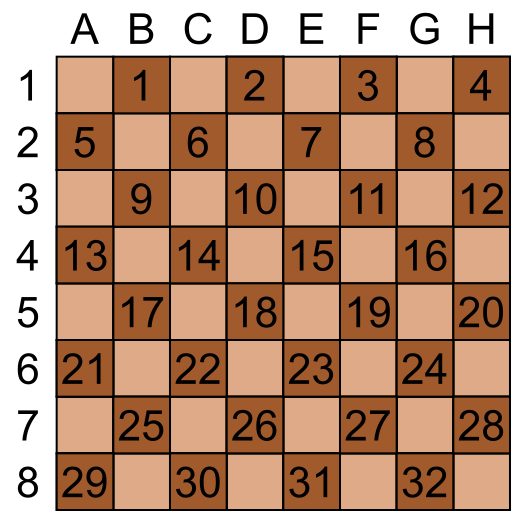
\includegraphics[scale=.6]{graphics/warcaby_planszaNumerowana.png}
    \caption{Numeracja pól i współrzędne planszy}
    \label{fig:numer}
\end{figure}


W przypadku podania błędnego wejścia, program poprosi gracza o ponowne wprowadzenie ruchu od zera. W momencie gdy rozgrywka miałaby się skończyć, program informuje o zwycięzcy i kończy działanie.

\subsection{Find}

Dostępne sygnatury wywołania programu:
\begin{itemize}
    \item Pierwsze uruchomienie algorytmu genetycznego (zalecane jeśli użytkownik chce utworzyć nową sesję algorytmu genetycznego od zera)
    \begin{enumerate}
        \item Liczebność populacji osobników [liczba naturalna podzielna przez 4]
        \item Liczba pojedynków osobnika w procesie selekcji [liczba naturalna, przy czym 0 oznacza pojedynek z każdym innym osobnikiem]
        \item Głębokość przeszukiwania w Minimaksie [liczba naturalna większa od zera]
        \item Współczynnik losowej selekcji osobników [liczba całkowita]
        \item Szansa na mutację [liczba wymierna z przedziału od~0 do~1]
        \item Rodzaj kryterium stopu [0 $\rightarrow$ czas (w sekundach); 1 $\rightarrow$ liczba iteracji]
        \item Limit dla kryterium stopu [liczba naturalna]
    \end{enumerate}
    \item Reaktywacja algorytmu genetycznego z wybranego pliku populacji
    \begin{enumerate}
        \item Nazwa pliku [ciąg znaków]
    \end{enumerate}
    \item Reaktywacja algorytmu genetycznego z ostatniego pliku populacji [BRAK ARGUMENTÓW]
    \vspace{1cm}
    \item Kontynuacja algorytmu genetycznego z nowymi parametrami
    \begin{enumerate}
        \item Nazwa pliku z którego należy wczytać populację [ciąg znaków]
        \item Liczba pojedynków osobnika w procesie selekcji [liczba naturalna, przy czym 0 oznacza pojedynek z każdym innym osobnikiem]
        \item Głębokość przeszukiwania w Minimaksie [liczba naturalna większa od zera]
        \item Współczynnik losowej selekcji osobników [liczba całkowita]
        \item Szansa na mutację [liczba wymierna między 0 a 1]
        \item Rodzaj kryterium stopu [0 $\rightarrow$ czas (w sekundach); 1 $\rightarrow$ liczba iteracji]
        \item Limit dla kryterium stopu [liczba naturalna]
    \end{enumerate}
\end{itemize}

Bezbłędne uruchomienie rozpocznie sesję algorytmu genetycznego z podanymi argumentami. W trakcie działania program operuje na plikach w katalogu \textit{heuristics} i jego podkatalogach: \textit{population} (pliki zapisanych populacji, z których można reaktywować sesje; program na bieżąco aktualizuje plik populacji) oraz \textit{output} (najlepiej przystosowany osobnik, tworzony w katalogu po osiągnięciu kryterium stopu). Oprócz tych podkatalogów istnieją również \textit{single} (katalog na samodzielne tworzenie plików ciągów wag) i~\textit{archive} (archiwum w którym można bezpiecznie zapisywać pliki ciągów wag), lecz program na tych dwóch podkatalogach nie wykonuje żadnych operacji oprócz ich stworzenia.

Sesja algorytmu genetycznego na bieżąco informuje o postępie - w każdej iteracji drukuje numer porządkowy obecnie ewaluowanej generacji oraz stosunek postępu do limitu we wcześniej podanym kryterium stopu (np. 5/100 generacji lub 100/2000 sekund). W razie niespodziewanego wcześniejszego zakończenia programu, możliwym jest odczyt argumentów sesji i postępu z pliku ostatniej populacji.

\subsection{Show}

Dostępne sygnatury wywołania programu:
\begin{itemize}
    \item Wydrukowanie ciągu wag z pliku osobnika
    \begin{enumerate}
        \item Ścieżka do pliku osobnika
    \end{enumerate}
\end{itemize}

Program drukuje listę opisanych parametrów z przydzielonymi im wagami z podanego pliku. Jest to użyteczne narzędzie do wglądu w wyniki sesji algorytmu genetycznego.

